%https://www.lama.univ-savoie.fr/mediawiki/index.php/G%C3%A9n%C3%A9ration_et_r%C3%A9solution_de_labyrinthes
% https://cpge-itc.github.io/itc1/5_graph/3_traversal/labyrinth/#animation-du-dfs
\exer{Génération et parcours de labyrinthe}
%\begin{flushright}
%
%\end{flushright}
\setcounter{numques}{0}


\subsection*{Génération d'un labyrinthe}

Soit une grille rectangulaire $n\times p$ constituée de $n$ lignes et de $p$ colonnes contenant toutes les arêtes possibles. On modélise cette grille par un graphe dont l'ensemble des sommets est donné par les couples $(i,j)$ tels que $i\in\llbracket 0,n \llbracket $ et $j\in\llbracket 0,p \llbracket $. Les voisins d'un sommet $(i,j)$ sont ceux situés en haut, en bas, à droite et à gauche s'ils existent (par exemple, le sommet $(0,0)$ a comme voisin les sommets $(0,1)$ et $(1,0)$).

\begin{center}
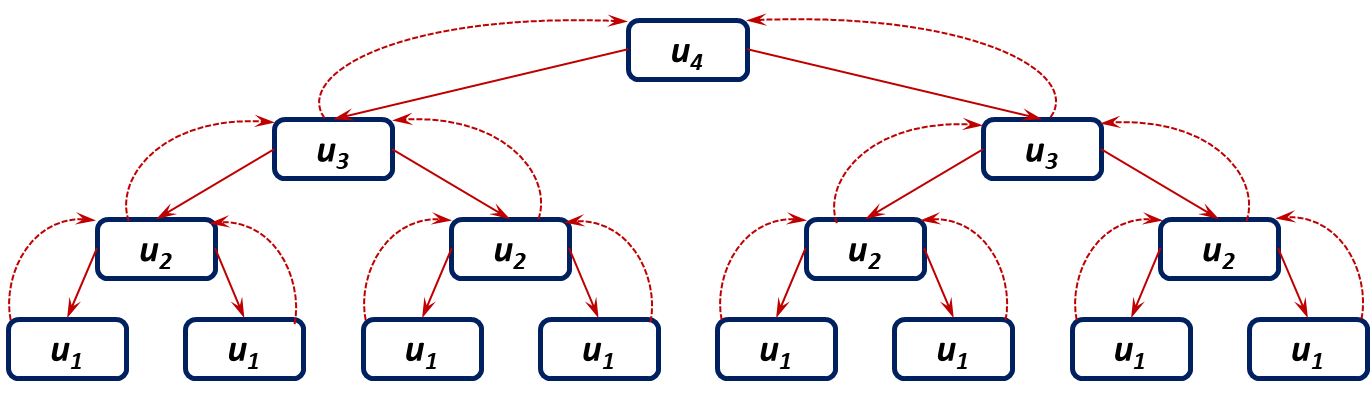
\includegraphics[width=7cm]{fig_01}
\end{center}

Le graphe est implémenté par un dictionnaire d'adjacence ou les clés sont les tuples, coordonnées d'un sommet. La valeur associée est une liste des sommet voisins. 


Ainsi, la grille $ 2 \times 2$ sera modélisée par le graphe suivant

\cde{\{(0,0):[(0,1),(1,0)], (0,1):[(0,0),(1,1)], (1,0):[(0,0),(1,1)], (1,1):[(0,1),(1,0)]\}}.
